% !TeX program = xelatex
\documentclass[a4paper,10pt]{article}

% ============================================================================
% កញ្ចប់សម្ភារៈសិក្សាបោះពុម្ព ស-ខ្មៅ (Printable Classroom Materials - Grade 8 2.4.3 POWQ)
% ត្រូវគ្នា ១០០% នឹង LS_Plan_POWQ.tex, Teaching_Scenario_POWQ.tex និង Teaching_Guideline_POWQ.tex
% ============================================================================
\usepackage[a4paper, left=1.0cm, right=1.0cm, top=0.75cm, bottom=1.05cm, footskip=0.55cm]{geometry}
\usepackage{amsmath, amssymb}
\usepackage{unicode-math}
\usepackage{fontspec}
\usepackage{array, colortbl}
\usepackage[table]{xcolor}
\usepackage{enumitem}
\usepackage{pifont}
\usepackage{fancyhdr}
\usepackage{lastpage}
\usepackage{tikz}
\usepackage[most]{tcolorbox}
\usetikzlibrary{calc, arrows.meta, decorations.markings, decorations.pathreplacing, positioning, babel}

% LaTeX 2025 compatibility guard
\makeatletter
\let\@expl@@@mark@update@singlecol@structures@@\relax
\makeatother

% ============================================================================
% ការកំណត់ពុម្ពអក្សរផ្លូវការ (Cross-Platform Khmer + Cambria Math + Times New Roman)
% ============================================================================
\providecommand{\NGSFindFonts}{%
  \IfFileExists{C:/Windows/Fonts/cambria.ttc}{%
    \def\NGSSysPath{C:/Windows/Fonts/}%
    \def\NGSUserPath{C:/Users/KIT/AppData/Local/Microsoft/Windows/Fonts/}%
  }{%
    \IfFileExists{./fonts/KhmerOSsiemreap.ttf}{\def\NGSSysPath{./fonts/}\def\NGSUserPath{./fonts/}}{%
    \IfFileExists{../fonts/KhmerOSsiemreap.ttf}{\def\NGSSysPath{../fonts/}\def\NGSUserPath{../fonts/}}{%
    \IfFileExists{../../fonts/KhmerOSsiemreap.ttf}{\def\NGSSysPath{../../fonts/}\def\NGSUserPath{../../fonts/}}{%
    \IfFileExists{../../../fonts/KhmerOSsiemreap.ttf}{\def\NGSSysPath{../../../fonts/}\def\NGSUserPath{../../../fonts/}}{%
    \IfFileExists{../../../../fonts/KhmerOSsiemreap.ttf}{\def\NGSSysPath{../../../../fonts/}\def\NGSUserPath{../../../../fonts/}}{%
    \IfFileExists{../../../../../fonts/KhmerOSsiemreap.ttf}{\def\NGSSysPath{../../../../../fonts/}\def\NGSUserPath{../../../../../fonts/}}{%
    \IfFileExists{../../../../../../fonts/KhmerOSsiemreap.ttf}{\def\NGSSysPath{../../../../../../fonts/}\def\NGSUserPath{../../../../../../fonts/}}{%
      \def\NGSSysPath{../../../../../../../fonts/}\def\NGSUserPath{../../../../../../../fonts/}%
    }}}}}}}%
  }%
}
\NGSFindFonts

\setmathfont[
  Path={\NGSSysPath},
  FontIndex=1,
  Scale=1.02
]{cambria.ttc}

\defaultfontfeatures{Ligatures=TeX}

\setmainfont[
  Path={\NGSUserPath},
  Extension=.ttf,
  Script=Khmer,
  BoldFont={KhmerOSsiemreap},
  BoldFeatures={FakeBold=1.8},
  ItalicFont={KhmerOSsiemreap},
  ItalicFeatures={FakeSlant=0.25},
  BoldItalicFont={KhmerOSsiemreap},
  BoldItalicFeatures={FakeBold=1.8, FakeSlant=0.25}
]{KhmerOSsiemreap}

\newfontfamily\muol[
  Path={\NGSUserPath},
  Extension=.ttf,
  Script=Khmer
]{KhmerOSmuollight}

\newfontfamily\TimesEn[
  Path={\NGSSysPath},
  Extension=.ttf,
  BoldFont={timesbd},
  ItalicFont={timesi},
  BoldItalicFont={timesbi}
]{times}

\newfontfamily\CalibriFont[
  Path={\NGSSysPath},
  Extension=.ttf
]{calibri}

\newfontfamily\Tacteing[
  Path={\NGSUserPath}
]{TACTENG.TTF}

\XeTeXlinebreaklocale "km"
\XeTeXlinebreakskip = 0pt plus 1pt minus 0.1pt

% ============================================================================
% ក្ដារពណ៌ ស-ខ្មៅ សុទ្ធសម្រាប់ការបោះពុម្ព (Strict Monochrome B&W Print Palette)
% ============================================================================
\definecolor{panelgray}{gray}{0.92} % ~gray!8
\definecolor{headgray}{gray}{0.85}  % ~gray!15
\definecolor{midgray}{gray}{0.75}   % ~gray!25
\definecolor{darkline}{gray}{0.35}  % ~gray!65

\pagestyle{fancy}
\fancyhf{}
\renewcommand{\headrulewidth}{0pt}
\fancyfoot[L]{\fontsize{7.2pt}{9.5pt}\selectfont អនុវិទ្យាល័យព្រះក្រសាំង \en{|} គ្រូ៖ ហុក ប៊ុនថែន \en{|} ២.៤.៣ ស្វ័យគុណនៃផលចែក (ស-ខ្មៅ) \en{|} ថ្ងៃចន្ទ ៧កើត ខែកត្តិក ឆ្នាំមមី អដ្ឋស័ក ព.ស. ២៥៧០ \en{|} ថ្ងៃចន្ទ ទី១៦ ខែវិច្ឆិកា ឆ្នាំ២០២៦}
\fancyfoot[R]{\fontsize{7.8pt}{9.5pt}\selectfont ទំព័រ \en{\thepage\ / \pageref{LastPage}}}

\setlength{\parindent}{0pt}
\setlength{\parskip}{0pt}
\setlength{\tabcolsep}{4pt}

% ============================================================================
% ម៉ាក្រូជំនួយ (Helper Macros)
% ============================================================================
\newcommand{\en}[1]{{\TimesEn #1}}
\newcommand{\enbf}[1]{{\TimesEn\bfseries #1}}
\newcommand{\unit}[1]{\,\text{\en{#1}}}
\newcommand{\cnum}[1]{\mbox{\fontsize{10pt}{12pt}\selectfont\ding{\numexpr181+#1\relax}}}
\newcommand{\cblank}{\tikz[baseline=-0.35ex]\draw[black, line width=0.8pt] (0,0) circle (0.17cm);}
\newcommand{\expbox}[1][0.38cm]{\,\tikz[baseline=-0.05ex]\draw[black, line width=0.65pt, fill=white] (0,0) rectangle (#1, 0.24cm);\,}
\newcommand{\expboxtight}[1][0.28cm]{\tikz[baseline=-0.05ex]\draw[black, line width=0.65pt, fill=white] (0,0) rectangle (#1, 0.22cm);}
\newcommand{\scissors}{\ding{34}}
\newcommand{\chkbox}{\tikz[baseline=-0.15ex]\draw[black, line width=0.85pt] (0,0) rectangle (0.23cm,0.23cm);}
\newcommand{\khmflourish}{{\Tacteing\fontsize{30pt}{13pt}\selectfont\raisebox{-4pt}{3}}}

\newcommand{\pagebanner}[2]{%
  \begin{tcolorbox}[
    enhanced, sharp corners, colback=headgray, colframe=black,
    boxrule=1.1pt, boxsep=1pt, top=2.5pt, bottom=2.5pt, left=6pt, right=6pt,
    after skip=4pt
  ]
    {\muol\fontsize{9.0pt}{13.2pt}\selectfont #1}\hfill{\fontsize{7.9pt}{11.2pt}\selectfont\textbf{#2}}
  \end{tcolorbox}%
}

\newcolumntype{L}[1]{>{\raggedright\arraybackslash}p{#1}}
\newcolumntype{C}[1]{>{\centering\arraybackslash}p{#1}}

\begin{document}
\fontsize{9.0pt}{13.0pt}\selectfont

% ============================================================================
% ទំព័រទី ១៖ សម្ភារៈ E2 ខ្នាតពិត 1:1 (ក្រឡា 5x5 cm + បន្ទះកាត់ 2x2 cm + POE 2A 4x4 cm + POE 2B)
% ============================================================================
\pagebanner{សម្ភារៈទី ១៖ បន្ទះកាត់ \enbf{E2} ខ្នាតពិត \enbf{1:1} ស្វ័យគុណនៃផលចែក \enbf{\&} ពិសោធន៍ \enbf{POE 2A--2B}}{ទំព័រ ១/៦ \en{-- E2 Explore}}

% --- ប្រអប់ព្រមានខ្នាតពិត & បន្ទះផ្ទៀង 5.00 cm (x=1cm, y=1cm) ---
\noindent
\begin{minipage}[c]{11.80cm}
  \begin{tcolorbox}[
    enhanced, sharp corners, colback=panelgray, colframe=black,
    boxrule=1.0pt, boxsep=1pt, top=2.5pt, bottom=2.5pt, left=5.5pt, right=5.5pt
  ]
    \fontsize{7.7pt}{10.6pt}\selectfont
    \textbf{សេចក្ដីណែនាំបោះពុម្ពខ្នាតពិត (\en{1:1 True Scale})៖} ត្រូវជ្រើស \textbf{\en{Scale: Actual Size 100\%} \en{--} ហាម \en{Fit to Page}} ដើម្បីឱ្យក្រឡា $5.00\times 5.00\unit{cm}$, បន្ទះកាត់ $2.00\times 2.00\unit{cm}$ និង \en{POE 2A} ($4.00\times 4.00\unit{cm}$) រក្សាខ្នាតពិត ១០០\%។\\[1.5pt]
    \textbf{ក្រុម ៣ នាក់៖} ផ្ទៀងបន្ទះ \en{5.00 cm} $\rightarrow$ ទស្សន៍ទាយ (\en{P}) $\rightarrow$ កាត់/តម្រៀបពិសោធន៍ (\en{O}) $\rightarrow$ ពន្យល់ (\en{E})។
  \end{tcolorbox}
\end{minipage}%
\hfill
\begin{minipage}[c]{6.90cm}
  \begin{tcolorbox}[
    enhanced, sharp corners, colback=white, colframe=black,
    boxrule=1.0pt, boxsep=1pt, top=2pt, bottom=2pt, left=4pt, right=4pt
  ]
    \centering
    {\fontsize{7.5pt}{9.5pt}\selectfont\textbf{បន្ទះផ្ទៀងខ្នាតពិត \en{5.00 cm} (\en{Actual Size 100\%})}}\\[1.5pt]
    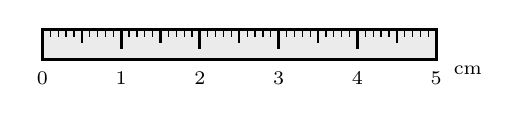
\begin{tikzpicture}[x=1cm, y=1cm, every node/.style={font=\scriptsize, text=black}]
      \draw[black, line width=1.1pt, fill=panelgray] (0,0) rectangle (5.0, 0.38);
      \foreach \m in {0,...,50}{
        \pgfmathsetmacro{\xval}{\m*0.1}
        \draw[black, line width=0.45pt] (\xval, 0.38) -- (\xval, 0.28);
      }
      \foreach \h in {0,0.5,...,5.0}{
        \draw[black, line width=0.8pt] (\h, 0.38) -- (\h, 0.21);
      }
      \foreach \c in {0,1,2,3,4,5}{
        \draw[black, line width=1.1pt] (\c, 0.38) -- (\c, 0.13);
        \node[below=1pt, font=\scriptsize] at (\c, 0.0) {\en{\c}};
      }
      \node[right=2pt, font=\scriptsize] at (5.03, -0.14) {\en{cm}};
    \end{tikzpicture}
  \end{tcolorbox}
\end{minipage}

\vspace{4pt}

% --- ផ្នែកទី ១៖ សកម្មភាព 1 — ក្រឡាឯកតា 5.00x5.00 cm + បន្ទះកាត់ 2.00x2.00 cm (1:1) + ផ្គុំកត្តា ទំ.១៨ ---
\textbf{\fontsize{8.5pt}{11.5pt}\selectfont ១. សកម្មភាព \en{1} (\en{1:1 True Scale}) ៖ ក្រឡាផ្ទៃឯកតា $5.00\times 5.00\unit{cm}$, បន្ទះកាត់ $2.00\times 2.00\unit{cm}$ និងផ្គុំកត្តា (ទំ.១៨)}

\vspace{3pt}
\noindent
\begin{minipage}[c]{6.80cm}
  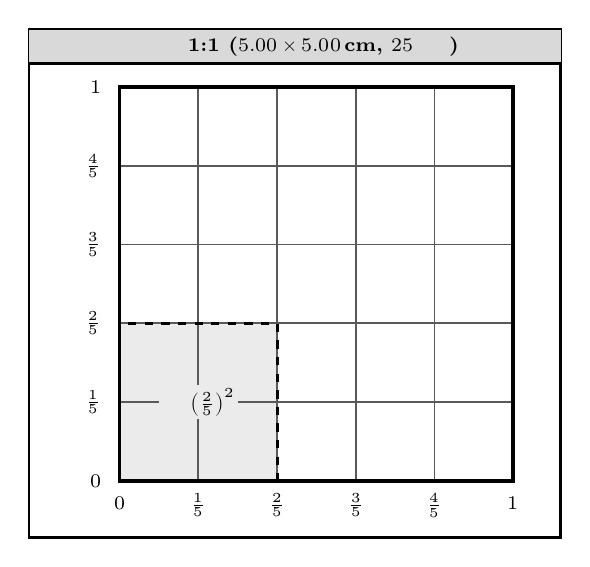
\begin{tikzpicture}[x=1cm, y=1cm, every node/.style={font=\scriptsize, text=black}]
    % Outer container: 6.75 cm x 6.45 cm
    \draw[black, line width=1.0pt] (0, 0) rectangle (6.75, 6.45);
    \fill[headgray] (0, 6.02) rectangle (6.75, 6.45);
    \draw[black, line width=0.8pt] (0, 6.02) -- (6.75, 6.02);
    \node[font=\scriptsize] at (3.375, 6.235) {\textbf{ក្រឡាឯកតា \en{1:1} ($5.00\times 5.00\unit{cm}$, $25$ ការ៉េ)}};

    % Exact 5.00 cm x 5.00 cm grid: origin (1.15, 0.72) -> (6.15, 5.72)
    \fill[panelgray] (1.15, 0.72) rectangle (3.15, 2.72);
    \foreach \k in {1,2,3,4}{
      \draw[darkline, line width=0.65pt] (1.15+\k, 0.72) -- (1.15+\k, 5.72);
      \draw[darkline, line width=0.65pt] (1.15, 0.72+\k) -- (6.15, 0.72+\k);
    }
    \draw[black, line width=1.35pt] (1.15, 0.72) rectangle (6.15, 5.72);
    \draw[black, dashed, line width=1.15pt] (1.15, 0.72) rectangle (3.15, 2.72);
    \node[fill=panelgray, inner sep=1pt, font=\scriptsize] at (2.15, 1.72) {ដាក់ $\left(\frac{2}{5}\right)^2$};

    % Bottom fraction labels along 0..1 (1 cm apart -> generous >=2.5mm clearance)
    \node[below=2pt, font=\scriptsize] at (1.15, 0.72) {$0$};
    \node[below=1pt, font=\scriptsize] at (2.15, 0.72) {$\frac{1}{5}$};
    \node[below=1pt, font=\scriptsize] at (3.15, 0.72) {$\frac{2}{5}$};
    \node[below=1pt, font=\scriptsize] at (4.15, 0.72) {$\frac{3}{5}$};
    \node[below=1pt, font=\scriptsize] at (5.15, 0.72) {$\frac{4}{5}$};
    \node[below=2pt, font=\scriptsize] at (6.15, 0.72) {$1$};

    % Left fraction labels along 0..1
    \node[left=3pt, font=\scriptsize] at (1.15, 0.72) {$0$};
    \node[left=3pt, font=\scriptsize] at (1.15, 1.72) {$\frac{1}{5}$};
    \node[left=3pt, font=\scriptsize] at (1.15, 2.72) {$\frac{2}{5}$};
    \node[left=3pt, font=\scriptsize] at (1.15, 3.72) {$\frac{3}{5}$};
    \node[left=3pt, font=\scriptsize] at (1.15, 4.72) {$\frac{4}{5}$};
    \node[left=3pt, font=\scriptsize] at (1.15, 5.72) {$1$};
  \end{tikzpicture}
\end{minipage}%
\hfill
\begin{minipage}[c]{11.95cm}
  % Top row: 1:1 Cut-out 2.00 cm x 2.00 cm tile + Instructions
  \noindent
  \begin{minipage}[c]{4.10cm}
    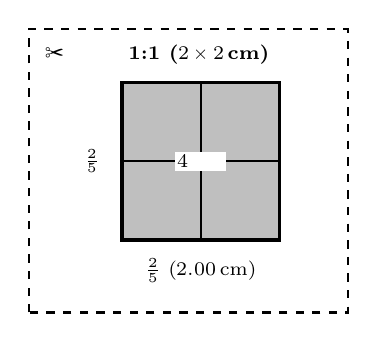
\begin{tikzpicture}[x=1cm, y=1cm, every node/.style={font=\scriptsize, text=black}]
      \draw[black, dashed, line width=0.95pt] (0, 0) rectangle (4.05, 3.60);
      \node[anchor=north west, font=\scriptsize] at (0.08, 3.52) {\scissors\ \textbf{កាត់បន្ទះ \en{1:1} ($2\times 2\unit{cm}$)}};
      % Exact 2.00 cm x 2.00 cm shaded tile: (1.18, 0.92) -> (3.18, 2.92)
      \fill[midgray] (1.18, 0.92) rectangle (3.18, 2.92);
      \draw[black, line width=0.8pt] (2.18, 0.92) -- (2.18, 2.92);
      \draw[black, line width=0.8pt] (1.18, 1.92) -- (3.18, 1.92);
      \draw[black, line width=1.35pt] (1.18, 0.92) rectangle (3.18, 2.92);
      \node[fill=white, inner sep=1pt, font=\scriptsize] at (2.18, 1.92) {$4$ ការ៉េ};
      \node[below=2pt, font=\scriptsize] at (2.18, 0.88) {$\frac{2}{5}$ ($2.00\unit{cm}$)};
      \node[left=3pt, font=\scriptsize] at (1.14, 1.92) {$\frac{2}{5}$};
    \end{tikzpicture}
  \end{minipage}%
  \hfill
  \begin{minipage}[c]{7.68cm}
    \begin{tcolorbox}[
      enhanced, sharp corners, colback=panelgray, colframe=black,
      boxrule=0.85pt, boxsep=1pt, top=4.5pt, bottom=4.5pt, left=5.5pt, right=5.5pt
    ]
      \raggedright\fontsize{7.6pt}{10.8pt}\selectfont
      \textbf{វិធីពិសោធន៍ \en{Act 1} (\en{1:1} -- ធុងកាត់បង្រួម $\frac{2}{5}\unit{m}$)៖}\\[2pt]
      \textbf{១.} កាត់ \scissors\ បន្ទះការ៉េ $2.00\times 2.00\unit{cm}$ ដាក់លើក្រឡា $5\times 5\unit{cm}$។\\[2pt]
      \textbf{២.} រាប់ផ្ទៃ៖ $\frac{2}{5}\times\frac{2}{5} \Rightarrow \left(\frac{2}{5}\right)^2 = \dfrac{\expbox}{\expbox} \neq \dfrac{4}{5}$ ($4$ ក្នុង $25$ ការ៉េ!)។\\[2pt]
      \textbf{៣.} បើជាគូប \en{E1}៖ ត្រូវប្ដូរទាំងភាគយកនិងភាគបែង $\left(\frac{2}{5}\right)^3$!
    \end{tcolorbox}
  \end{minipage}

  \vspace{5pt}
  % Bottom row: Textbook p. 18 factor-pairing card
  \begin{tcolorbox}[
    enhanced, sharp corners, colback=white, colframe=black,
    boxrule=0.95pt, boxsep=1pt, top=3.5pt, bottom=3.5pt, left=5.5pt, right=5.5pt,
    title={\textbf{ការផ្គុំកត្តា (ឧទាហរណ៍ ទំ.១៨) ៖ សរសេរដោយប្រើនិទស្សន្តតែមួយ}},
    colbacktitle=headgray, coltitle=black, fonttitle=\fontsize{7.9pt}{10.6pt}\selectfont
  ]
    \raggedright\fontsize{7.8pt}{11.4pt}\selectfont
    \textbf{ក.} $\dfrac{2^3}{5^3} = \dfrac{\overbrace{2\times 2\times 2}^{3\text{ កត្តា}}}{\underbrace{5\times 5\times 5}_{3\text{ កត្តា}}} = \underbrace{\left(\dfrac{2}{5}\right)\left(\dfrac{2}{5}\right)\left(\dfrac{2}{5}\right)}_{3\text{ កត្តា}} = \left(\dfrac{2}{5}\right)^{\expbox}$ \quad\chkbox\\[3pt]
    \textbf{ខ.} $\dfrac{a^n}{b^n} = \dfrac{\overbrace{a\cdot a\cdot\ldots a}^{n\text{ កត្តា}}}{\underbrace{b\cdot b\cdot\ldots b}_{n\text{ កត្តា}}} = \underbrace{\left(\dfrac{a}{b}\right)\cdot\left(\dfrac{a}{b}\right)\cdot\ldots\left(\dfrac{a}{b}\right)}_{n\text{ កត្តា}} = \left(\dfrac{a}{b}\right)^{\expbox}$ ($b\neq 0$) \quad\chkbox
  \end{tcolorbox}
\end{minipage}

\vspace{5pt}

% --- ផ្នែកទី ២៖ សកម្មភាព 2 (POE 2A: 4x4 cm 1:1 & POE 2B: អន្ទាក់ផលបូក) ---
\textbf{\fontsize{8.5pt}{11.5pt}\selectfont ២. សកម្មភាព \en{2} (\en{POE 2A \& 2B}) ៖ អន្ទាក់ភ្លេចភាគបែង \en{1:1} និងអន្ទាក់ចែកចាយលើផលបូក}

\vspace{3pt}
\noindent
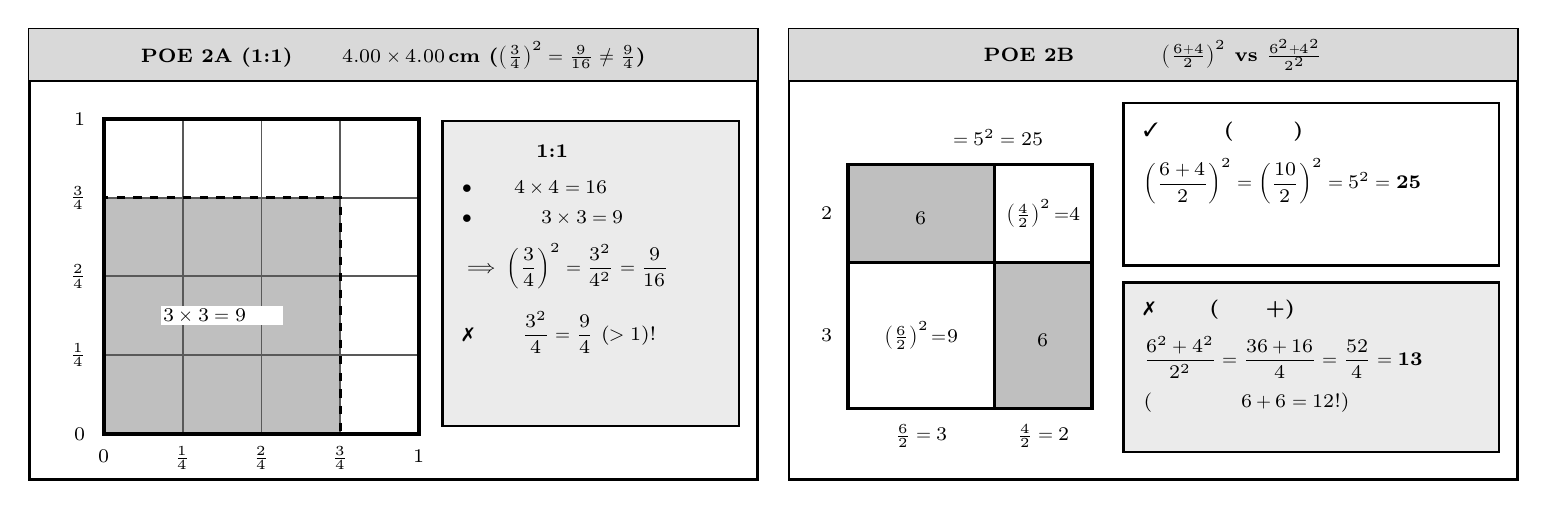
\begin{tikzpicture}[x=1cm, y=1cm, every node/.style={font=\scriptsize, text=black}]
  % === Panel POE 2A: Exact 4.00 cm x 4.00 cm 1:1 Grid (0..9.25, height 5.72) ===
  \begin{scope}[shift={(0,0)}]
    \draw[black, line width=1.05pt] (0, 0) rectangle (9.25, 5.72);
    \fill[headgray] (0, 5.06) rectangle (9.25, 5.72);
    \draw[black, line width=0.85pt] (0, 5.06) -- (9.25, 5.06);
    \node[font=\scriptsize] at (4.625, 5.39) {\textbf{\en{POE 2A (1:1)}៖ ក្រឡា $4.00\times 4.00\unit{cm}$ ($\left(\frac{3}{4}\right)^2 = \frac{9}{16} \neq \frac{9}{4}$)}};

    % 4.00 cm x 4.00 cm grid: (0.95, 0.58) -> (4.95, 4.58)
    \fill[midgray] (0.95, 0.58) rectangle (3.95, 3.58);
    \foreach \k in {1,2,3}{
      \draw[darkline, line width=0.65pt] (0.95+\k, 0.58) -- (0.95+\k, 4.58);
      \draw[darkline, line width=0.65pt] (0.95, 0.58+\k) -- (4.95, 0.58+\k);
    }
    \draw[black, line width=1.35pt] (0.95, 0.58) rectangle (4.95, 4.58);
    \draw[black, dashed, line width=1.15pt] (0.95, 0.58) rectangle (3.95, 3.58);
    \node[fill=white, inner sep=1pt, font=\scriptsize] at (2.45, 2.08) {$3\times 3 = 9$ ការ៉េ};

    % Bottom ticks
    \node[below=2pt, font=\scriptsize] at (0.95, 0.58) {$0$};
    \node[below=1pt, font=\scriptsize] at (1.95, 0.58) {$\frac{1}{4}$};
    \node[below=1pt, font=\scriptsize] at (2.95, 0.58) {$\frac{2}{4}$};
    \node[below=1pt, font=\scriptsize] at (3.95, 0.58) {$\frac{3}{4}$};
    \node[below=2pt, font=\scriptsize] at (4.95, 0.58) {$1$};

    % Left ticks
    \node[left=3pt, font=\scriptsize] at (0.95, 0.58) {$0$};
    \node[left=3pt, font=\scriptsize] at (0.95, 1.58) {$\frac{1}{4}$};
    \node[left=3pt, font=\scriptsize] at (0.95, 2.58) {$\frac{2}{4}$};
    \node[left=3pt, font=\scriptsize] at (0.95, 3.58) {$\frac{3}{4}$};
    \node[left=3pt, font=\scriptsize] at (0.95, 4.58) {$1$};

    % Right explanation box inside POE 2A
    \draw[black, line width=0.8pt, fill=panelgray] (5.25, 0.68) rectangle (9.02, 4.55);
    \node[anchor=north west, align=left, font=\scriptsize] at (5.38, 4.38)
      {\textbf{ពិនិត្យក្រឡា \en{1:1}៖}\\[5pt]
       $\bullet$ សរុប៖ $4\times 4 = 16$ ការ៉េ\\[3pt]
       $\bullet$ ឈូសប្រផេះ៖ $3\times 3 = 9$ ការ៉េ\\[6pt]
       $\implies \left(\dfrac{3}{4}\right)^2 = \dfrac{3^2}{4^2} = \dfrac{9}{16}$\\[7pt]
       \textbf{\ding{55}\ មិនមែន} $\dfrac{3^2}{4} = \dfrac{9}{4}$ ($> 1$)!};
  \end{scope}

  % === Panel POE 2B: Additive Non-Distributivity Trap (9.65..18.90, height 5.72) ===
  \begin{scope}[shift={(9.65,0)}]
    \draw[black, line width=1.05pt] (0, 0) rectangle (9.25, 5.72);
    \fill[headgray] (0, 5.06) rectangle (9.25, 5.72);
    \draw[black, line width=0.85pt] (0, 5.06) -- (9.25, 5.06);
    \node[font=\scriptsize] at (4.625, 5.39) {\textbf{\en{POE 2B}៖ អន្ទាក់ផលបូក $\left(\frac{6+4}{2}\right)^2$ \en{vs} $\frac{6^2+4^2}{2^2}$}};

    % Left sub-diagram: 5x5 grid showing (3+2)^2 = 25 vs 3^2+2^2 = 13
    \begin{scope}[shift={(0.75, 0.90)}]
      % Scale each unit = 0.62 cm -> 5 units = 3.10 cm
      \fill[midgray] (0, 1.86) rectangle (1.86, 3.10); % 3x2 missing cross-bar
      \fill[midgray] (1.86, 0) rectangle (3.10, 1.86); % 2x3 missing cross-bar
      \fill[white] (0, 0) rectangle (1.86, 1.86);      % 3^2 = 9
      \fill[white] (1.86, 1.86) rectangle (3.10, 3.10); % 2^2 = 4
      \draw[black, line width=1.25pt] (0, 0) rectangle (3.10, 3.10);
      \draw[black, line width=0.95pt] (1.86, 0) -- (1.86, 3.10);
      \draw[black, line width=0.95pt] (0, 1.86) -- (3.10, 1.86);
      \node[font=\scriptsize] at (0.93, 0.93) {$\left(\frac{6}{2}\right)^2{=}9$};
      \node[font=\scriptsize] at (2.48, 2.48) {$\left(\frac{4}{2}\right)^2{=}4$};
      \node[align=center, font=\scriptsize] at (0.93, 2.48) {បាត់\\$6$};
      \node[align=center, font=\scriptsize] at (2.48, 0.93) {បាត់\\$6$};
      \node[below=2pt, font=\scriptsize] at (0.93, 0) {$\frac{6}{2}=3$};
      \node[below=2pt, font=\scriptsize] at (2.48, 0) {$\frac{4}{2}=2$};
      \node[left=2pt, font=\scriptsize] at (0, 0.93) {$3$};
      \node[left=2pt, font=\scriptsize] at (0, 2.48) {$2$};
      \node[above=2pt, font=\scriptsize] at (1.55, 3.14) {ការ៉េសរុប $= 5^2 = 25$};
    \end{scope}

    % Right calculation comparison boxes
    \draw[black, line width=0.9pt, fill=white] (4.25, 2.72) rectangle (9.02, 4.78);
    \node[anchor=north west, align=left, font=\scriptsize] at (4.38, 4.66)
      {\textbf{\ding{51}\ វិធីត្រូវ (បូកក្នុងមុន)៖}\\[5pt]
       $\left(\dfrac{6+4}{2}\right)^2 = \left(\dfrac{10}{2}\right)^2 = 5^2 = \mathbf{25}$};

    \draw[black, line width=0.9pt, fill=panelgray] (4.25, 0.35) rectangle (9.02, 2.50);
    \node[anchor=north west, align=left, font=\scriptsize] at (4.38, 2.40)
      {\textbf{\ding{55}\ វិធីខុស (បំបែកលើ \en{+})៖}\\[5pt]
       $\dfrac{6^2+4^2}{2^2} = \dfrac{36+16}{4} = \dfrac{52}{4} = \mathbf{13}$\\[4pt]
       (បាត់ផ្នែកប្រផេះ $6+6 = 12$!)};
  \end{scope}
\end{tikzpicture}

\vspace{7pt}

% --- តារាងកំណត់ត្រា POE (Predict - Observe - Explain) ---
\begin{tcolorbox}[
  enhanced, sharp corners, colback=white, colframe=black,
  boxrule=1.0pt, boxsep=1pt, top=6pt, bottom=6pt, left=6pt, right=6pt
]
  \raggedright\fontsize{8.0pt}{11.6pt}\selectfont
  \textbf{\en{P} -- ទស្សន៍ទាយមុនពិសោធន៍ (\en{Predict})៖}\\[3pt]
  \textbf{១) \en{POE 2A}៖} តើ $\left(\dfrac{3}{4}\right)^2$ ស្មើប៉ុន្មាន? \quad \chkbox~$\dfrac{9}{4}$ \quad \chkbox~$\dfrac{9}{16}$ \qquad
  \textbf{២) \en{POE 2B}៖} តើ $\left(\dfrac{6+4}{2}\right)^2 = \dfrac{6^2+4^2}{2^2}$ ឬទេ? \quad \chkbox~ស្មើ \quad \chkbox~មិនស្មើ\\[5pt]

  \textbf{\en{O} -- តារាងសង្កេត និងផ្ទៀងផ្ទាត់ (\en{Observe})៖}\\[3pt]
  \renewcommand{\arraystretch}{1.32}
  \begin{tabular}{|L{3.75cm}|L{9.45cm}|L{4.10cm}|}
    \hline
    \cellcolor{headgray}\textbf{ផ្ទាំងពិសោធន៍ \en{POE}} & \cellcolor{headgray}\textbf{រង្វាស់ខ្នាតពិត \en{1:1} និងការគណនា} & \cellcolor{headgray}\textbf{លទ្ធផលសង្កេត} \\ \hline
    \textbf{\en{POE 2A}}៖ ក្រឡា $4\times 4\unit{cm}$ & សរុប $\underline{\hspace{0.45cm}}$ ការ៉េ \en{|} ឈូសប្រផេះ $\underline{\hspace{0.45cm}}$ ការ៉េ ($3\times 3$) & \chkbox~$\left(\dfrac{3}{4}\right)^2 = \dfrac{9}{16} \neq \dfrac{9}{4}$! \\ \hline
    \textbf{\en{POE 2B}}៖ អន្ទាក់ផលបូក & $\left(\dfrac{6+4}{2}\right)^2 = 5^2 = \underline{\hspace{0.55cm}}$ \en{|} $\dfrac{6^2+4^2}{2^2} = \dfrac{52}{4} = \underline{\hspace{0.55cm}}$ & \chkbox~$25 \neq 13$ (ហាមបំបែកលើ \en{+})! \\ \hline
  \end{tabular}\\[6pt]

  \textbf{\en{E} -- ពន្យល់សន្និដ្ឋាន (\en{Explain})៖} ស្វ័យគុណចែកចាយគ្រប់កត្តាទាំងភាគយកនិងភាគបែងលើ\textbf{ផលចែក} $\left(\dfrac{a}{b}\right)^n = \dfrac{a^{\expbox}}{b^{\expbox}}$ ($a,b\neq 0$) ប៉ុន្តែ\textbf{ហាម}ចែកចាយលើផលបូក ឬផលដក $(a\pm b)^n \neq a^n\pm b^n$៖ $\underline{\hspace{4.2cm}}$
\end{tcolorbox}

\clearpage

% ============================================================================
% ទំព័រទី ២៖ E4 Elaborate — ២ ប័ណ្ណ "លំហាត់គំរូទី 1 (ទំ.១៨) & បញ្ច្រាស គ" + [tracing] + EIA 30s
% ============================================================================
\pagebanner{សម្ភារៈទី ២៖ កាត \enbf{E4} «\enbf{3} ជំហាន \enbf{[}ចង្អុលអូស\enbf{]}» \enbf{(}គំរូទី \enbf{1} ទំ\enbf{.}១៨ \enbf{\&} បញ្ច្រាស\enbf{)}}{ទំព័រ ២/៦ \en{-- E4} (កាត់ ២ ប័ណ្ណ \scissors)}

\newcommand{\eFourCardPOWQ}[1]{%
\begin{tcolorbox}[
  enhanced, sharp corners, colback=white, colframe=white,
  borderline={1.0pt}{0pt}{black, dashed},
  boxsep=1pt, top=5pt, bottom=5pt, left=5.5pt, right=5.5pt
]
  \begin{tcolorbox}[
    enhanced, sharp corners, colback=headgray, colframe=black,
    boxrule=0.8pt, boxsep=1pt, top=3pt, bottom=3pt, left=5pt, right=5pt, after skip=5pt
  ]
    \fontsize{8.2pt}{11.2pt}\selectfont
    \textbf{\scissors\ កាត \en{E4} (#1) \en{--} លំហាត់គំរូទី \en{1} (សៀវភៅទំ.១៨) \& ផ្គុំបញ្ច្រាស គ} \hfill ក្រុម៖ $\underline{\hspace{2.6cm}}$
  \end{tcolorbox}

  \noindent
  \begin{minipage}[t]{7.30cm}
    \vspace{0pt}
    % Outside-In 3-Step [tracing] Diagram
    \begin{center}
    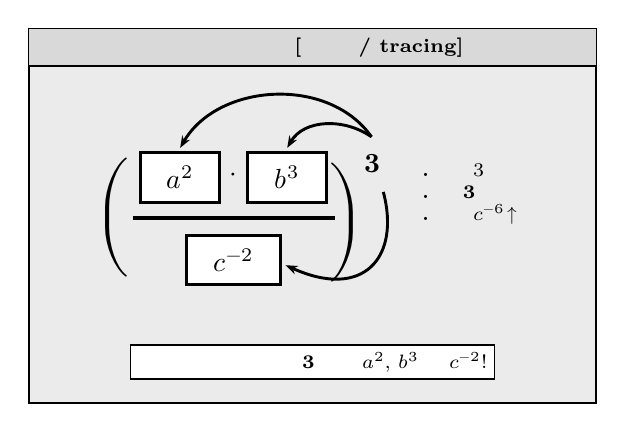
\begin{tikzpicture}[x=1cm, y=1cm, every node/.style={font=\scriptsize, text=black}]
      \draw[black, line width=0.95pt, fill=panelgray] (0, 0) rectangle (7.20, 4.75);
      \fill[headgray] (0, 4.28) rectangle (7.20, 4.75);
      \draw[black, line width=0.8pt] (0, 4.28) -- (7.20, 4.28);
      \node[font=\scriptsize] at (3.60, 4.515) {\textbf{ដ្យាក្រាមពីក្រៅចូលក្នុង \en{[}ចង្អុលអូស \en{/ tracing]}}};

      % Big parenthesis & boxed numerator/denominator factors
      \node[font=\Large] at (1.05, 2.35) {$\Bigg($};
      \draw[black, line width=1.1pt, fill=white] (1.42, 2.55) rectangle (2.42, 3.18);
      \node[font=\normalsize] at (1.92, 2.865) {$a^2$};
      \node[font=\normalsize] at (2.60, 2.865) {$\cdot$};
      \draw[black, line width=1.1pt, fill=white] (2.78, 2.55) rectangle (3.78, 3.18);
      \node[font=\normalsize] at (3.28, 2.865) {$b^3$};

      % Fraction bar
      \draw[black, line width=1.25pt] (1.32, 2.35) -- (3.88, 2.35);

      % Denominator boxed factor c^-2
      \draw[black, line width=1.1pt, fill=white] (2.00, 1.50) rectangle (3.20, 2.13);
      \node[font=\normalsize] at (2.60, 1.815) {$c^{-2}$};

      \node[font=\Large] at (4.15, 2.35) {$\Bigg)^{\mathbf{3}}$};

      % Tracing arrows from outer exponent 3 to EVERY factor (a^2, b^3, c^-2)
      \draw[black, line width=1.05pt, -{Stealth[length=1.5mm]}] (4.35, 3.38) to[out=125, in=60] (1.92, 3.24);
      \draw[black, line width=1.05pt, -{Stealth[length=1.5mm]}] (4.35, 3.38) to[out=145, in=60] (3.28, 3.24);
      \draw[black, line width=1.05pt, -{Stealth[length=1.5mm]}] (4.50, 2.68) .. controls (4.72, 1.85) and (4.25, 1.30) .. (3.26, 1.75);

      % Step cues on the right
      \node[anchor=west, align=left, font=\scriptsize] at (4.80, 2.65)
        {\textbf{១.} ព័ទ្ធ $3$ កត្តា\\
         \textbf{២.} អូស $\mathbf{3}$ គ្រប់\\
         \textbf{៣.} ប្ដូរ $c^{-6}\!\uparrow$};

      \node[draw=black, line width=0.65pt, fill=white, inner sep=2.5pt, font=\scriptsize] at (3.60, 0.52)
        {ប្រើម្រាមដៃអូសពីនិទស្សន្តក្រៅ $\mathbf{3}$ ទៅទាំង $a^2$, $b^3$ និង $c^{-2}$!};
    \end{tikzpicture}
    \end{center}
    \vspace{4pt}
    \begin{tcolorbox}[enhanced, sharp corners, colback=panelgray, colframe=black, boxrule=0.75pt, boxsep=1pt, top=3.5pt, bottom=3.5pt, left=5pt, right=5pt]
      \raggedright\fontsize{7.4pt}{10.4pt}\selectfont
      \textbf{ពិនិត្យក្រោយ (\en{EIA} ៣០ វិនាទី)៖}\\
      \textbf{១)} ហេតុអ្វី $\dfrac{1}{c^{-6}} = \mathbf{+}c^6$ មិនមែន $-c^6$? (ច្រាសគុណ \cnum{4} មិនប្ដូរសញ្ញា $+$/$-$ ឡើយ!)\\
      \textbf{២)} ក្នុង \textbf{គ} ហេតុអ្វីផ្គុំ $\frac{6^4}{3^4}=\left(\frac{6}{3}\right)^4$ មុនគណនា? (ប្រើ \cnum{1} ពីរទិស!)
    \end{tcolorbox}
  \end{minipage}\hfill
  \begin{minipage}[t]{10.45cm}
    \vspace{0pt}
    \begin{tcolorbox}[enhanced, sharp corners, colback=white, colframe=black, boxrule=0.85pt, boxsep=1pt, top=4pt, bottom=4pt, left=4.5pt, right=4.5pt]
      \raggedright\fontsize{7.4pt}{11.0pt}\selectfont
      {\fontsize{7.7pt}{11.2pt}\selectfont\textbf{ជំហាន ១--៣៖ ដោះស្រាយលំហាត់គំរូទី \en{1} (ទំ.១៨) \& បញ្ច្រាស គ ៖}}\\[4pt]
      \textbf{ក.} $\left(\dfrac{3}{4}\right)^3 = \dfrac{3^{\expbox}}{4^{\expbox}} = \dfrac{\underline{\hspace{0.55cm}}}{\underline{\hspace{0.55cm}}}$ \hfill \mbox{\chkbox\ (\cblank)}\\[6pt]
      \textbf{ខ.} $\left(\dfrac{a^2 b^3}{c^{-2}}\right)^3 = \dfrac{(a^2)^{\expbox[0.30cm]}(b^3)^{\expbox[0.30cm]}}{(c^{-2})^{\expbox[0.30cm]}} = \dfrac{a^{\expbox[0.30cm]} b^{\expbox[0.30cm]}}{c^{\expbox[0.30cm]}} = a^{\expbox[0.30cm]} b^{\expbox[0.30cm]} c^{\expbox[0.30cm]}\,(c\!\neq\!0)$ \hfill \mbox{\chkbox\ (\cblank,\!\cblank,\!\cblank)}\\[6pt]
      \textbf{គ. (ផ្គុំបញ្ច្រាសលាយ)៖} {\thickmuskip=2.4mu\medmuskip=1.8mu$\dfrac{6^4}{3^4}\cdot(2^{-1})^2 = \left(\dfrac{\underline{\hspace{0.34cm}}}{\underline{\hspace{0.34cm}}}\right)^{\expboxtight} \cdot 2^{\expboxtight} = 2^{\expboxtight} \cdot 2^{\expboxtight} = 2^{\expboxtight} = \underline{\hspace{0.38cm}}$} \hfill \mbox{\chkbox\ (\cblank,\cblank)}
    \end{tcolorbox}
    \vspace{5pt}
    \begin{tcolorbox}[enhanced, sharp corners, colback=panelgray, colframe=black, boxrule=0.85pt, boxsep=1pt, top=4pt, bottom=4pt, left=5pt, right=5pt]
      \raggedright\fontsize{7.5pt}{10.8pt}\selectfont
      \textbf{តារាងត្រួតពិនិត្យជំហាន ស-ខ្មៅ (\en{[tracing]} + ហេតុផល \cnum{1}--\cnum{5})៖}\\[3pt]
      {\setlength{\tabcolsep}{3pt}\renewcommand{\arraystretch}{1.35}%
      \begin{tabular}{|L{1.85cm}|L{3.40cm}|L{3.90cm}|}
        \hline
        \cellcolor{headgray}\textbf{លំហាត់} & \cellcolor{headgray}\textbf{ដាន \en{[tracing]} ត្រូវពិនិត្យ} & \cellcolor{headgray}\textbf{សំអាង \cnum{1}--\cnum{5} \& លទ្ធផល} \\ \hline
        \textbf{ក.} $(3/4)^3$ & និទស្សន្ត $3$ ចូលទាំង $3$ និង $4$ & \cnum{1} $\Rightarrow 27/64$ \\ \hline
        \textbf{ខ.} $(a^2b^3/c^{-2})^3$ & អូស $3$ ចូល $a^2, b^3, c^{-2}$ & \cnum{1}, \cnum{3}, \cnum{4} $\Rightarrow a^6b^9c^6$ \\ \hline
        \textbf{គ.} $\frac{6^4}{3^4}(2^{-1})^2$ & ផ្គុំ $6^4/3^4$ និងគុណ $(-1)\times 2$ & \cnum{1}, \cnum{3}, \cnum{4} $\Rightarrow 4$ \\ \hline
      \end{tabular}}
    \end{tcolorbox}
    \vspace{4pt}
    \raggedright{\fontsize{6.9pt}{9.6pt}\selectfont
    \textbf{ធនាគារ \cnum{1}--\cnum{5}៖} \cnum{1} $(a/b)^n=a^n/b^n$ (ពីរទិស) \en{|} \cnum{2} $(ab)^n=a^nb^n$ \en{|} \cnum{3} $(a^m)^n=a^{mn}$ \en{|} \cnum{4} $a^m a^n, a^{-n}, 1/c^{-n}=c^n$ \en{|} \cnum{5} $(-x)^{\text{គូ/សេស}}$\par}
  \end{minipage}
\end{tcolorbox}%
}

\vspace{2pt}
\eFourCardPOWQ{ប័ណ្ណទី ១}

\vspace{10pt}
\noindent\scissors\ \dotfill\ \textbf{កាត់តាមស្នាមចុចចែកជា ២ ប័ណ្ណ (\en{Cut Along Dashed Line})} \dotfill\ \scissors
\vspace{10pt}

\eFourCardPOWQ{ប័ណ្ណទី ២}

\clearpage

% ============================================================================
% ទំព័រទី ៣៖ E5 Evaluate — "សន្លឹកសហការ ៣ តួនាទី (Proof Relay)" — ប្រតិបត្តិ ទំ.១៨ + Task 3 + បិទ E1
% ============================================================================
\pagebanner{សម្ភារៈទី ៣៖ សន្លឹក \enbf{E5} សហការ ៣ តួនាទី \enbf{(Proof Relay --} ប្រតិបត្តិ ទំ\enbf{.}១៨ \enbf{\&} បិទ \enbf{E1)}}{ទំព័រ ៣/៦ \en{-- E5 Evaluate} (កាត់ ២ សន្លឹក \scissors)}

\newcommand{\eFiveSheetPOWQ}[1]{%
\begin{tcolorbox}[
  enhanced, sharp corners, colback=white, colframe=white,
  borderline={1.0pt}{0pt}{black, dashed},
  boxsep=1pt, top=3pt, bottom=3pt, left=4.5pt, right=4.5pt
]
  \begin{tcolorbox}[
    enhanced, sharp corners, colback=headgray, colframe=black,
    boxrule=0.8pt, boxsep=1pt, top=2.5pt, bottom=2.5pt, left=5pt, right=5pt, after skip=3.5pt
  ]
    \fontsize{7.4pt}{10.0pt}\selectfont
    \textbf{\scissors\ សន្លឹកសហការ ៣ តួនាទី (#1) \en{--} ប្រតិបត្តិ (ទំ.១៨) \& សំយោគលក្ខណៈទាំង ៣} \hfill ក្រុម៖ $\underline{\hspace{2.2cm}}$
  \end{tcolorbox}

  \renewcommand{\arraystretch}{1.08}
  {\centering\setlength{\tabcolsep}{3.5pt}%
  \begin{tabular}{|L{5.55cm}|L{6.85cm}|L{5.20cm}|}
    \hline
    \cellcolor{panelgray}\centering\arraybackslash\fontsize{7.3pt}{9.6pt}\selectfont\textbf{តួនាទី ១៖ អ្នកគូសដាន \en{[tracing]} \en{\& Pause-Ask!}}\newline {\fontsize{6.6pt}{8.6pt}\selectfont ព័ទ្ធកត្តា \& ចង្អុលអូសនិទស្សន្ត ($x,y,b,c\neq 0$)} &
    \cellcolor{panelgray}\centering\arraybackslash\fontsize{7.3pt}{9.6pt}\selectfont\textbf{តួនាទី ២៖ អ្នកភ្ជាប់ហេតុផល \cnum{1}--\cnum{4} \& គណនា}\newline {\fontsize{6.6pt}{8.6pt}\selectfont អនុវត្តលក្ខណៈទាំង ៣ និងចុះលេខ \cnum{1}--\cnum{5}} &
    \cellcolor{panelgray}\centering\arraybackslash\fontsize{7.3pt}{9.6pt}\selectfont\textbf{តួនាទី ៣៖ អ្នកត្រួតពិនិត្យសញ្ញា និងលំដាប់ \cnum{5}}\newline {\fontsize{6.6pt}{8.6pt}\selectfont \en{Pause-Review!} \en{\&} បិទបេសកកម្មធុងទឹក \en{E1}} \\ \hline

    % --- Column 1: Factor Mapper [tracing] ---
    {\centering
    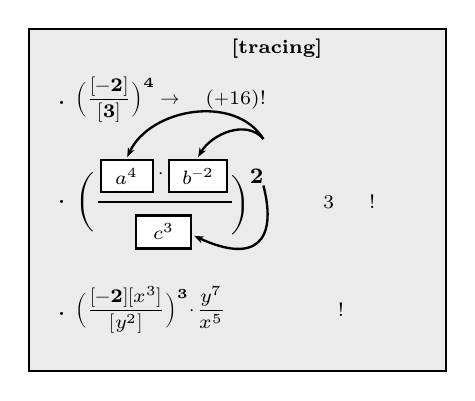
\begin{tikzpicture}[baseline={([yshift=-1.2ex]current bounding box.north)}, x=1cm, y=1cm, every node/.style={font=\scriptsize, text=black}]
      \draw[black, line width=0.8pt, fill=panelgray] (0, 0) rectangle (5.30, 4.35);
      \node[font=\scriptsize] at (2.65, 4.10) {\textbf{ដានព័ទ្ធកត្តា \en{[tracing]}}};

      % Task 1 visual
      \node[anchor=west, font=\scriptsize] at (0.18, 3.45) {\textbf{១.} $\Big(\dfrac{[\mathbf{-2}]}{[\mathbf{3}]}\Big)^{\mathbf{4}} \to$ \text{គូ ($+16$)!}};

      % Task 2 visual with clean boxed factors & non-crossing arrows
      \node[anchor=west, font=\scriptsize] at (0.18, 2.15) {\textbf{២.}};
      \node[font=\large] at (0.72, 2.15) {$\Big($};
      \draw[black, line width=0.85pt, fill=white] (0.92, 2.28) rectangle (1.58, 2.68);
      \node[font=\scriptsize] at (1.25, 2.48) {$a^4$};
      \node[font=\scriptsize] at (1.68, 2.48) {$\cdot$};
      \draw[black, line width=0.85pt, fill=white] (1.78, 2.28) rectangle (2.52, 2.68);
      \node[font=\scriptsize] at (2.15, 2.48) {$b^{-2}$};
      \draw[black, line width=1.0pt] (0.88, 2.15) -- (2.58, 2.15);
      \draw[black, line width=0.85pt, fill=white] (1.36, 1.56) rectangle (2.06, 1.98);
      \node[font=\scriptsize] at (1.71, 1.77) {$c^3$};
      \node[font=\large] at (2.78, 2.15) {$\Big)^{\mathbf{2}}$};

      \draw[black, line width=0.85pt, -{Stealth[length=1.2mm]}] (2.98, 2.95) to[out=122, in=65] (1.25, 2.72);
      \draw[black, line width=0.85pt, -{Stealth[length=1.2mm]}] (2.98, 2.95) to[out=130, in=60] (2.15, 2.72);
      \draw[black, line width=0.85pt, -{Stealth[length=1.2mm]}] (2.98, 2.36) .. controls (3.16, 1.65) and (2.88, 1.36) .. (2.10, 1.72);
      \node[anchor=west, font=\scriptsize] at (3.25, 2.15) {ទាំង $3$ កត្តា!};

      % Task 3 visual
      \node[anchor=west, font=\scriptsize] at (0.18, 0.78) {\textbf{៣.} $\Big(\dfrac{[\mathbf{-2}][x^3]}{[y^2]}\Big)^{\mathbf{3}}\!\cdot\!\dfrac{y^7}{x^5}$};
      \node[anchor=west, font=\scriptsize] at (3.25, 0.78) {បំបែកមុន!};
    \end{tikzpicture}\par\vspace{4pt}}
    \fontsize{7.1pt}{9.8pt}\selectfont
    \chkbox\ \textbf{\en{Pause-Ask!}} ហេតុអ្វី $(-2)^4 = +16$ តែ $(-2)^3 = -8$? ហើយហេតុអ្វី $b^{-4}$ ត្រូវចុះភាគបែង?
    &
    % --- Column 2: Warrant Connector 1-4 ---
    \fontsize{7.3pt}{10.5pt}\selectfont
    \textbf{១. ប្រតិបត្តិ ក (ទំ.១៨)៖}\par\vspace{1.5pt}
    $\left(\dfrac{-2}{3}\right)^4 = \dfrac{(-2)^{\expbox}}{3^{\expbox}} = \dfrac{\underline{\hspace{0.48cm}}}{\underline{\hspace{0.48cm}}}$ \hfill (\cblank, \cblank)\par\vspace{5pt}

    \textbf{២. ប្រតិបត្តិ ខ (ទំ.១៨) ($b,c\neq 0$)៖}\par\vspace{1.5pt}
    $\left(\dfrac{a^4\cdot b^{-2}}{c^3}\right)^2 = \dfrac{(a^4)^{\expbox}(b^{-2})^{\expbox}}{(c^3)^{\expbox}}$ \hfill (\cblank, \cblank)\par\vspace{2pt}
    \hspace*{1.2em} $= \dfrac{a^{\expbox} b^{\expbox}}{c^{\expbox}} = \dfrac{a^{\expbox}}{b^{\expbox} c^{\expbox}}$ \hfill (\cblank, \cblank)\par\vspace{5pt}

    \textbf{៣. សំយោគលក្ខណៈទាំង ៣ ($x,y\neq 0$)៖}\par\vspace{1.5pt}
    $\left(\dfrac{-2x^3}{y^2}\right)^3\cdot\dfrac{y^7}{x^5} = \dfrac{(-2)^{\expbox} x^{\expbox}}{y^{\expbox}}\cdot\dfrac{y^7}{x^5}$ \hfill (\cblank, \cblank)\par\vspace{2pt}
    \hspace*{1.2em} $= \underline{\hspace{0.60cm}} \cdot x^{\expbox} \cdot y^{\expbox} = \underline{\hspace{1.45cm}}$ \hfill (\cblank, \cblank)
    &
    % --- Column 3: Sign & Order Auditor (5), Pause-Review!, E1 Closure ---
    \fontsize{7.0pt}{9.8pt}\selectfont
    \chkbox\ \textbf{\en{Pause-Review!}} ផ្ទៀង៖\par\vspace{2pt}
    ១) សញ្ញា \cnum{5}៖ $(-2)^4=+16$ (គូ), $(-2)^3=-8$ (សេស)!\par\vspace{1.5pt}
    ២) $b^{-4}=\frac{1}{b^4}$ ចុះភាគបែង (\cnum{4}) និង $b,c,x,y\neq 0$?\par\vspace{1.5pt}
    ៣) មានហេតុផល \cnum{1}--\cnum{5} គ្រប់ជំហាន!\par\vspace{4pt}
    \begin{tcolorbox}[enhanced, sharp corners, colback=panelgray, colframe=black, boxrule=0.7pt, boxsep=1pt, top=3pt, bottom=3pt, left=4pt, right=4pt]
      \raggedright\fontsize{6.9pt}{9.7pt}\selectfont
      \textbf{បិទបេសកកម្ម \en{E1} (ធុងស្តុកទឹក)៖}\\
      ជ្រុងធុង $1\unit{m} \to \frac{2}{5}\unit{m}$ មានមាឌ៖\\
      $V = \left(\dfrac{2}{5}\right)^3 = \dfrac{2^{\expbox}}{5^{\expbox}} = \dfrac{\underline{\hspace{0.35cm}}}{\underline{\hspace{0.45cm}}}\unit{m}^3$ ($< 1\unit{m}^3$!)\\[2pt]
      \chkbox\ ហត្ថលេខាក្រុម៖ $\underline{\hspace{1.6cm}}$
    \end{tcolorbox}
    \\ \hline
  \end{tabular}\par}
  \vspace{3pt}
  {\centering\fontsize{6.9pt}{9.4pt}\selectfont \textbf{ធនាគារ \cnum{1}--\cnum{5}៖} \cnum{1} $(a/b)^n=a^n/b^n$ \en{|} \cnum{2} $(ab)^n=a^nb^n$ \en{|} \cnum{3} $(a^m)^n=a^{mn}$ \en{|} \cnum{4} $a^m a^n, a^{-n}, 1/c^{-n}=c^n$ \en{|} \cnum{5} $(-x)^{\text{គូ/សេស}}, (a\pm b)^n\neq a^n\pm b^n$\par}
\end{tcolorbox}%
}

\vspace{2pt}
\eFiveSheetPOWQ{សន្លឹកទី ១}

\vspace{6pt}
\noindent\scissors\ \dotfill\ \textbf{កាត់តាមស្នាមចុចចែកជា ២ សន្លឹក (\en{Cut Along Dashed Line})} \dotfill\ \scissors
\vspace{6pt}

\eFiveSheetPOWQ{សន្លឹកទី ២}

\clearpage

% ============================================================================
% ទំព័រទី ៤៖ ផ្ទាំងសំអាងមេរៀន ២.៤.៣ — Hub-and-Spoke & ធនាគារ ①–⑤ & អន្ទាក់ហាមទាំង ៣
% ============================================================================
\begin{tcolorbox}[
  enhanced, sharp corners, colback=white, colframe=black,
  boxrule=1.5pt, borderline={0.6pt}{2.2pt}{black},
  boxsep=1pt, top=12pt, bottom=12pt, left=6.5pt, right=6.5pt
]
  \begin{center}
    {\fontsize{8.2pt}{11.2pt}\selectfont មន្ទីរអប់រំ យុវជន និងកីឡា ខេត្តកំពង់ធំ \en{|} ការិយាល័យអប់រំ យុវជន និងកីឡា ស្រុកកំពង់ស្វាយ \en{|} អនុវិទ្យាល័យព្រះក្រសាំង}\\[3.5pt]
    {\muol\fontsize{11.2pt}{16.6pt}\selectfont ផ្ទាំងសំអាងមេរៀន ២\enbf{.}៤\enbf{.}៣៖ ស្វ័យគុណនៃផលចែក និងលក្ខណៈទាំង ៣ \enbf{(}\cnum{1}\enbf{--}\cnum{5}\enbf{)}}\\[3.5pt]
    {\fontsize{7.5pt}{10.5pt}\selectfont គណិតវិទ្យា ថ្នាក់ទី៨ \en{--} មេរៀនទី២ (ទំ.១៧\en{--}១៨) \en{|} គ្រូបង្រៀន៖ ហុក ប៊ុនថែន \en{|} ថ្ងៃចន្ទ ៧កើត ខែកត្តិក ឆ្នាំមមី អដ្ឋស័ក ព.ស. ២៥៧០ (ថ្ងៃទី១៦ ខែវិច្ឆិកា ឆ្នាំ២០២៦)}\\[4.5pt]
    \khmflourish
  \end{center}
  \vspace{9pt}

  % --- ផ្នែកទី ១៖ Hub-and-Spoke (ឆ្វេង) & ប្រអប់ជាទូទៅ ៤.៣ (ស្ដាំ) ---
  \noindent
  \begin{minipage}[t]{9.20cm}
    \begin{tcolorbox}[
      enhanced, sharp corners, colback=white, colframe=black,
      boxrule=0.95pt, boxsep=1pt, equal height group=posterTopPOWQ,
      top=6pt, bottom=6pt, left=5pt, right=5pt,
      title={\textbf{រចនាសម្ព័ន្ធ \en{Hub-and-Spoke} ជុំវិញនិយមន័យគោល $x^n$}},
      colbacktitle=headgray, coltitle=black, fonttitle=\fontsize{8.3pt}{11.4pt}\selectfont
    ]
      \centering
      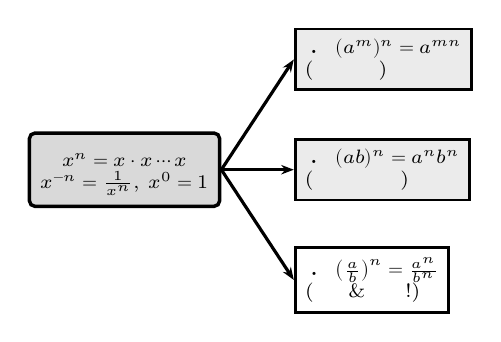
\begin{tikzpicture}[x=1cm, y=1cm, every node/.style={font=\scriptsize, text=black}]
        % Central Hub
        \node[draw=black, line width=1.25pt, fill=headgray, rounded corners=2pt, align=center, inner sep=4pt] (hub) at (1.55, 2.05)
          {\textbf{គោលស្នូល}\\$x^n = x\cdot x\cdots x$\\$x^{-n}=\frac{1}{x^n},\; x^0=1$};

        % Three Spokes radiating rightwards
        \node[draw=black, line width=1.0pt, fill=panelgray, align=left, inner sep=3.5pt, anchor=west] (s1) at (3.70, 3.45)
          {\textbf{៤.១៖} $(a^m)^n = a^{mn}$\\(គុណនិទស្សន្ត)};
        \node[draw=black, line width=1.0pt, fill=panelgray, align=left, inner sep=3.5pt, anchor=west] (s2) at (3.70, 2.05)
          {\textbf{៤.២៖} $(ab)^n = a^n b^n$\\(ចែកគ្រប់កត្តាគុណ)};
        \node[draw=black, line width=1.15pt, fill=white, align=left, inner sep=3.5pt, anchor=west] (s3) at (3.70, 0.65)
          {\textbf{៤.៣៖} $\left(\frac{a}{b}\right)^n = \frac{a^n}{b^n}$\\(ភាគយក \& ភាគបែង!)};

        % Bold spoke arrows
        \draw[black, line width=1.15pt, -{Stealth[length=1.6mm]}] (hub.east) -- (s1.west);
        \draw[black, line width=1.15pt, -{Stealth[length=1.6mm]}] (hub.east) -- (s2.west);
        \draw[black, line width=1.15pt, -{Stealth[length=1.6mm]}] (hub.east) -- (s3.west);
      \end{tikzpicture}
    \end{tcolorbox}
  \end{minipage}\hfill
  \begin{minipage}[t]{8.45cm}
    \begin{tcolorbox}[
      enhanced, sharp corners, colback=panelgray, colframe=black,
      boxrule=0.95pt, boxsep=1pt, equal height group=posterTopPOWQ,
      top=6pt, bottom=6pt, left=5.5pt, right=5.5pt,
      title={\textbf{៤.៣ ស្វ័យគុណនៃផលចែក (ទំ.១៨) \& ច្បាប់ច្រាស}},
      colbacktitle=headgray, coltitle=black, fonttitle=\fontsize{8.3pt}{11.4pt}\selectfont
    ]
      \raggedright\fontsize{8.0pt}{11.8pt}\selectfont
      \textbf{ជាទូទៅ៖} បើ $a, b$ ជាចំនួនសនិទានខុសពីសូន្យ និង $n$ ជាចំនួនគត់រ៉ឺឡាទីបខុសពីសូន្យ គេបាន៖
      \[
        \left(\dfrac{a}{b}\right)^n = \dfrac{a^n}{b^n}
      \]
      $\bullet$ \textbf{ពីរទិស៖} $\left(\dfrac{a}{b}\right)^n = \dfrac{a^n}{b^n} \iff \dfrac{a^n}{b^n} = \left(\dfrac{a}{b}\right)^n$\\[3pt]
      $\bullet$ \textbf{ច្រាសនិទស្សន្តដក៖} $\left(\dfrac{a}{b}\right)^{-n} = \dfrac{a^{-n}}{b^{-n}} = \dfrac{b^n}{a^n} = \left(\dfrac{b}{a}\right)^n$ ($a,b\neq 0$)\\[3pt]
      $\bullet$ \textbf{រូបភាព ១:១៖} $\left(\dfrac{2}{5}\right)^2 = \dfrac{4}{25} \neq \dfrac{4}{5}$ ($4$ ក្នុង $25$ ការ៉េ)
    \end{tcolorbox}
  \end{minipage}

  \vspace{11pt}

  % --- ផ្នែកទី ២៖ តារាងធនាគារហេតុផល ①–⑤ (Word-for-Word ១០០% នឹង Research_Brief & LS_Plan) ---
  \fontsize{7.9pt}{11.4pt}\selectfont
  \renewcommand{\arraystretch}{1.82}
  \begin{tabular}{|C{0.70cm}|L{3.95cm}|L{6.55cm}|C{4.95cm}|}
    \hline
    \cellcolor{headgray}\textbf{លេខ} &
    \cellcolor{headgray}\centering\arraybackslash\textbf{ឈ្មោះហេតុផល (\en{Warrant})} &
    \cellcolor{headgray}\centering\arraybackslash\textbf{រូបមន្ត និងលក្ខខណ្ឌកំណត់} &
    \cellcolor{headgray}\centering\arraybackslash\textbf{ដ្យាក្រាម \en{[tracing]} ស-ខ្មៅ} \\ \hline

    \cnum{1} &
    \textbf{ស្វ័យគុណនៃផលចែក (៤.៣ ពីរទិស \& ច្រាស)} &
    $\left(\dfrac{a}{b}\right)^n = \dfrac{a^n}{b^n} \iff \dfrac{a^n}{b^n} = \left(\dfrac{a}{b}\right)^n$ \newline និង $\left(\dfrac{a}{b}\right)^{-n} = \left(\dfrac{b}{a}\right)^n$ ($a,b\neq 0$) &
    \raisebox{-0.35\height}{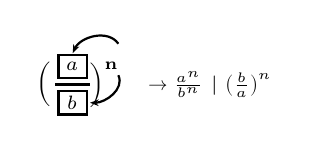
\begin{tikzpicture}[x=1cm, y=1cm, every node/.style={font=\scriptsize, text=black}]
      \node[font=\small] at (-0.18, 0.36) {$\Big($};
      \draw[black, line width=0.8pt] (0.00, 0.44) rectangle (0.36, 0.74);
      \node at (0.18, 0.59) {$a$};
      \draw[black, line width=0.9pt] (-0.04, 0.36) -- (0.40, 0.36);
      \draw[black, line width=0.8pt] (0.00, -0.02) rectangle (0.36, 0.28);
      \node at (0.18, 0.13) {$b$};
      \node[font=\small] at (0.58, 0.36) {$\Big)^{\mathbf{n}}$};
      \draw[black, line width=0.8pt, -{Stealth[length=1.1mm]}] (0.76, 0.88) to[out=125, in=65] (0.18, 0.76);
      \draw[black, line width=0.8pt, -{Stealth[length=1.1mm]}] (0.76, 0.48) to[out=-65, in=0] (0.40, 0.13);
      \node[right=2pt, font=\scriptsize] at (0.95, 0.36) {$\to \frac{a^n}{b^n}$ \en{|} $\big(\frac{b}{a}\big)^n$};
    \end{tikzpicture}} \\ \hline

    \cnum{2} &
    \textbf{ស្វ័យគុណនៃផលគុណ (៤.២)} &
    $(a\cdot b)^n = a^n\cdot b^n$ \newline \textit{(ចែកចាយគ្រប់កត្តារួមទាំងមេគុណលេខ; $a,b\neq 0$ បើ $n<0$)} &
    \raisebox{-0.35\height}{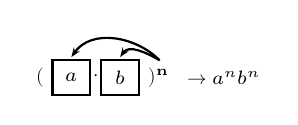
\begin{tikzpicture}[x=1cm, y=1cm, every node/.style={font=\scriptsize, text=black}]
      \draw[black, line width=0.85pt] (0, 0.04) rectangle (0.48, 0.48);
      \draw[black, line width=0.85pt] (0.62, 0.04) rectangle (1.10, 0.48);
      \node at (0.24, 0.26) {$a$}; \node at (0.55, 0.26) {$\cdot$}; \node at (0.86, 0.26) {$b$};
      \node at (-0.15, 0.26) {$($}; \node at (1.35, 0.26) {$)^{\mathbf{n}}$};
      \draw[black, line width=0.8pt, -{Stealth[length=1.2mm]}] (1.36, 0.48) to[out=135, in=55] (0.24, 0.52);
      \draw[black, line width=0.8pt, -{Stealth[length=1.2mm]}] (1.36, 0.48) to[out=150, in=55] (0.86, 0.52);
      \node[right=2pt, font=\scriptsize] at (1.52, 0.26) {$\to a^n b^n$};
    \end{tikzpicture}} \\ \hline

    \cnum{3} &
    \textbf{ស្វ័យគុណនៃស្វ័យគុណ (៤.១)} &
    $(a^m)^n = a^{mn}$ \newline \textit{(គុណនិទស្សន្តនឹងនិទស្សន្ត មិនមែនបូកទេ! $a\neq 0$ បើ $m,n<0$)} &
    \raisebox{-0.35\height}{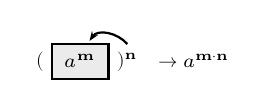
\begin{tikzpicture}[x=1cm, y=1cm, every node/.style={font=\scriptsize, text=black}]
      \draw[black, line width=0.85pt, fill=panelgray] (0, 0.04) rectangle (0.72, 0.48);
      \node at (0.36, 0.26) {$a^{\mathbf{m}}$};
      \node at (-0.14, 0.26) {$($}; \node at (0.96, 0.26) {$)^{\mathbf{n}}$};
      \draw[black, line width=0.8pt, -{Stealth[length=1.2mm]}] (0.96, 0.48) to[out=130, in=55] (0.48, 0.52);
      \node[right=2pt, font=\scriptsize] at (1.16, 0.26) {$\to a^{\mathbf{m\cdot n}}$};
    \end{tikzpicture}} \\ \hline

    \cnum{4} &
    \textbf{ច្បាប់គោលដូចគ្នា សូន្យ \& និទស្សន្តដក} &
    $a^m a^n = a^{m+n},\;\; \dfrac{a^m}{a^n} = a^{m-n},\;\; a^0 = 1,$ \newline $a^{-n} = \dfrac{1}{a^n} \iff \dfrac{1}{c^{-n}} = c^n$ ($a, c\neq 0$) &
    \raisebox{-0.35\height}{\begin{tikzpicture}[x=1cm, y=1cm, every node/.style={font=\scriptsize, text=black}]
      \node at (0.45, 0.28) {$\dfrac{1}{c^{-n}}$};
      \draw[black, line width=0.85pt, -{Stealth[length=1.2mm]}] (0.90, 0.14) to[out=35, in=-135] (1.45, 0.42);
      \node[right=2pt, font=\scriptsize] at (1.48, 0.28) {$+c^n$ (ឡើងលើ)};
    \end{tikzpicture}} \\ \hline

    \cnum{5} &
    \textbf{ភាពគូ/សេសសញ្ញាដក \& ដែនវង់ក្រចក} &
    $(-x)^{\text{គូ}} = +x^{\text{គូ}},\;\; (-x)^{\text{សេស}} = -x^{\text{សេស}},$ \newline $(a\pm b)^n \neq a^n\pm b^n$ និង $-c(ab)^n \neq (-cab)^n$ &
    \raisebox{-0.35\height}{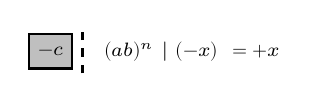
\begin{tikzpicture}[x=1cm, y=1cm, every node/.style={font=\scriptsize, text=black}]
      \draw[black, line width=0.85pt, fill=midgray] (0, 0.04) rectangle (0.55, 0.48);
      \node at (0.275, 0.26) {$-c$};
      \draw[black, dashed, line width=1.1pt] (0.68, -0.02) -- (0.68, 0.54);
      \node[right=2pt, font=\scriptsize] at (0.76, 0.26) {$(ab)^n$ \en{|} $(-x)^{\text{គូ}}=+x^{\text{គូ}}$};
    \end{tikzpicture}} \\ \hline
  \end{tabular}

  \vspace{11pt}

  % --- ផ្នែកទី ៣៖ ប្រអប់ព្រមាន "ប្រយ័ត្នអន្ទាក់ហាមទាំង ៣ (Forbidden Traps)" ---
  \begin{tcolorbox}[
    enhanced, sharp corners, colback=white, colframe=black,
    boxrule=1.15pt, boxsep=1pt, top=8pt, bottom=8pt, left=6.5pt, right=6.5pt,
    title={\ding{55}\ \textbf{ប្រយ័ត្នអន្ទាក់ហាមទាំង ៣ (\en{Forbidden Traps} -- កំហុសញឹកញាប់បំផុតក្នុងថ្នាក់ទី៨)}},
    colbacktitle=midgray, coltitle=black, fonttitle=\fontsize{8.8pt}{12.0pt}\selectfont
  ]
    \raggedright\fontsize{8.1pt}{12.4pt}\selectfont
    \textbf{១. ហាមចែកចាយស្វ័យគុណលើផលបូក/ដក៖} $(a \pm b)^n \neq a^n \pm b^n$ \quad (ឧ. $\left(\frac{6+4}{2}\right)^2 = 25 \neq \frac{6^2+4^2}{2^2} = 13$; ចែកបានតែផលគុណ \& ផលចែក!)\\[6pt]
    \textbf{២. ហាមច្រឡំសញ្ញាដកក្រៅវង់ក្រចក៖} $-a^n \neq (-a)^n$ \quad (ពេល $n$ គូ ឧ. $-3^2 = -9$ តែ $(-3)^2 = +9$; $-2(a^{-3}b^5)^2 = -\frac{2b^{10}}{a^6}$!)\\[6pt]
    \textbf{៣. ហាមប្ដូរសញ្ញាពេលលើកភាគបែងស្វ័យគុណដក៖} $\dfrac{1}{c^{-n}} = \mathbf{+}c^n \neq -c^n$ \quad (និទស្សន្តដកប្រាប់ពី\textbf{ទីតាំងច្រាស} មិនមែនសញ្ញាមេគុណទេ!)
  \end{tcolorbox}

  \vspace{10pt}
  \begin{tcolorbox}[
    enhanced, sharp corners, colback=panelgray, colframe=black,
    boxrule=0.75pt, boxsep=1pt, top=6pt, bottom=6pt, left=6pt, right=6pt
  ]
    \centering\fontsize{7.9pt}{11.2pt}\selectfont
    \textbf{គោលការណ៍ប្រើផ្ទាំងសំអាង (\en{E3--E5})៖} រាល់ជំហានដោះស្រាយក្នុង \textbf{លំហាត់គំរូ (ទំ.១៨)}, \textbf{ប្រតិបត្តិ} និង \textbf{កិច្ចការផ្ទះ (ទំ.២៥--២៦)} ត្រូវចុះលេខហេតុផល \cnum{1}--\cnum{5} ភ្ជាប់ជានិច្ច!
  \end{tcolorbox}
\end{tcolorbox}

\clearpage

% ============================================================================
% ទំព័រទី ៥៖ កាតវិនិច្ឆ័យរហ័ស E5 (កាត A–D លើ (-3x^2 / y^-4)^2) + Teacher Key & Exit Ticket 3 សំណួរ
% ============================================================================
\pagebanner{សម្ភារៈទី ៥៖ កាតវិនិច្ឆ័យរហ័ស «កាត \enbf{A--D}» \enbf{\&} សំបុត្រចេញរហ័ស \enbf{E5}}{ទំព័រ ៥/៦ \en{-- E5 Evaluate}}

{\fontsize{8.5pt}{11.8pt}\selectfont
\textbf{សំណួរចម្បង (\en{E5} លើកកាត \en{A--D} ឬបង្ហាញម្រាមដៃ \en{1--4})៖} «សម្រួលកន្សោម $\left(\dfrac{-3x^2}{y^{-4}}\right)^2$ ($x, y \neq 0$) \en{--} តើកាតមួយណា\textbf{ត្រឹមត្រូវ (\ding{51})}?»}

\vspace{6pt}

% --- ជួរទី ១៖ កាត A & កាត B ---
\noindent
\begin{tcolorbox}[
  enhanced, sharp corners, colback=white, colframe=white,
  borderline={1.0pt}{0pt}{black, dashed},
  width=9.25cm, equal height group=powqfoilrow1, nobeforeafter,
  boxsep=1pt, top=6pt, bottom=6pt, left=6pt, right=6pt
]
  \noindent\colorbox{black}{\textcolor{white}{\Large\textbf{\en{ A }}}}\hspace{0.22cm}{\fontsize{9.0pt}{12.0pt}\selectfont\textbf{កាត \en{A} ៖ លទ្ធផលទម្រង់ប្រភាគ}}\par\vspace{6pt}
  \begin{center}
    {\fontsize{17.5pt}{21pt}\selectfont $\displaystyle \left(\frac{-3x^2}{y^{-4}}\right)^2 \;=\; \frac{9x^4}{y^{-4}}$}
  \end{center}
  \vspace{4pt}
  \begin{center}
  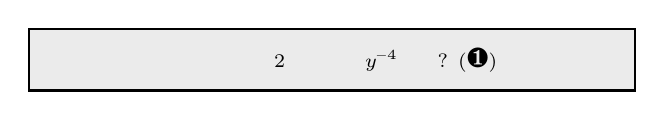
\begin{tikzpicture}[x=1cm, y=1cm, every node/.style={font=\scriptsize, text=black}]
    \draw[black, line width=0.9pt, fill=panelgray] (0,0) rectangle (7.7, 0.78);
    \node at (3.85, 0.39) {ផ្ទៀង៖ តើនិទស្សន្ត $2$ ចែកឱ្យភាគបែង $y^{-4}$ ដែរឬទេ? (\cnum{1})};
  \end{tikzpicture}
  \end{center}
  \vspace{3pt}
  {\centering\fontsize{7.8pt}{10.5pt}\selectfont ហេតុផល / លេខ \cnum{1}--\cnum{5}៖ $\underline{\hspace{4.5cm}}$\par}
  \vfill
  \begin{tcolorbox}[enhanced, sharp corners, colback=panelgray, colframe=black, boxrule=0.8pt, boxsep=1pt, top=4pt, bottom=4pt, left=4pt, right=4pt]
    \centering\fontsize{8.5pt}{11.5pt}\selectfont
    \textbf{វិនិច្ឆ័យ៖} \quad \chkbox~ពិត (\ding{51}) \qquad \chkbox~ខុស (\ding{55})
  \end{tcolorbox}
\end{tcolorbox}%
\hfill
\begin{tcolorbox}[
  enhanced, sharp corners, colback=white, colframe=white,
  borderline={1.0pt}{0pt}{black, dashed},
  width=9.25cm, equal height group=powqfoilrow1, nobeforeafter,
  boxsep=1pt, top=6pt, bottom=6pt, left=6pt, right=6pt
]
  \noindent\colorbox{black}{\textcolor{white}{\Large\textbf{\en{ B }}}}\hspace{0.22cm}{\fontsize{9.0pt}{12.0pt}\selectfont\textbf{កាត \en{B} ៖ លទ្ធផលផលគុណគ្មានភាគបែង}}\par\vspace{6pt}
  \begin{center}
    {\fontsize{17.5pt}{21pt}\selectfont $\displaystyle \left(\frac{-3x^2}{y^{-4}}\right)^2 \;=\; 9x^4y^2$}
  \end{center}
  \vspace{4pt}
  \begin{center}
  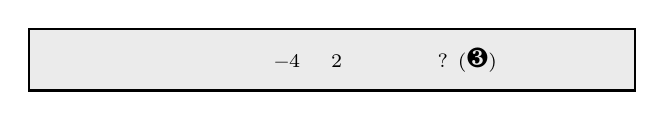
\begin{tikzpicture}[x=1cm, y=1cm, every node/.style={font=\scriptsize, text=black}]
    \draw[black, line width=0.9pt, fill=panelgray] (0,0) rectangle (7.7, 0.78);
    \node at (3.85, 0.39) {ផ្ទៀង៖ តើនិទស្សន្ត $-4$ និង $2$ ត្រូវ \textbf{គុណ} ឬ \textbf{បូក}? (\cnum{3})};
  \end{tikzpicture}
  \end{center}
  \vspace{3pt}
  {\centering\fontsize{7.8pt}{10.5pt}\selectfont ហេតុផល / លេខ \cnum{1}--\cnum{5}៖ $\underline{\hspace{4.5cm}}$\par}
  \vfill
  \begin{tcolorbox}[enhanced, sharp corners, colback=panelgray, colframe=black, boxrule=0.8pt, boxsep=1pt, top=4pt, bottom=4pt, left=4pt, right=4pt]
    \centering\fontsize{8.5pt}{11.5pt}\selectfont
    \textbf{វិនិច្ឆ័យ៖} \quad \chkbox~ពិត (\ding{51}) \qquad \chkbox~ខុស (\ding{55})
  \end{tcolorbox}
\end{tcolorbox}

\vspace{7pt}

% --- ជួរទី ២៖ កាត C & កាត D ---
\noindent
\begin{tcolorbox}[
  enhanced, sharp corners, colback=white, colframe=white,
  borderline={1.0pt}{0pt}{black, dashed},
  width=9.25cm, equal height group=powqfoilrow2, nobeforeafter,
  boxsep=1pt, top=6pt, bottom=6pt, left=6pt, right=6pt
]
  \noindent\colorbox{black}{\textcolor{white}{\Large\textbf{\en{ C }}}}\hspace{0.22cm}{\fontsize{9.0pt}{12.0pt}\selectfont\textbf{កាត \en{C} ៖ លទ្ធផលផលគុណគ្មានភាគបែង}}\par\vspace{6pt}
  \begin{center}
    {\fontsize{17.5pt}{21pt}\selectfont $\displaystyle \left(\frac{-3x^2}{y^{-4}}\right)^2 \;=\; 9x^4y^8$}
  \end{center}
  \vspace{4pt}
  \begin{center}
  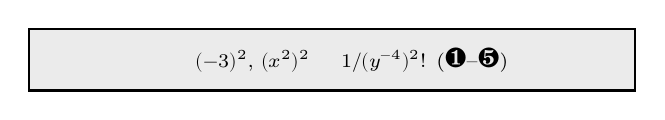
\begin{tikzpicture}[x=1cm, y=1cm, every node/.style={font=\scriptsize, text=black}]
    \draw[black, line width=0.9pt, fill=panelgray] (0,0) rectangle (7.7, 0.78);
    \node at (3.85, 0.39) {ផ្ទៀង៖ $(-3)^2$, $(x^2)^2$ និង $1/(y^{-4})^2$! (\cnum{1}--\cnum{5})};
  \end{tikzpicture}
  \end{center}
  \vspace{3pt}
  {\centering\fontsize{7.8pt}{10.5pt}\selectfont ហេតុផល / លេខ \cnum{1}--\cnum{5}៖ $\underline{\hspace{4.5cm}}$\par}
  \vfill
  \begin{tcolorbox}[enhanced, sharp corners, colback=panelgray, colframe=black, boxrule=0.8pt, boxsep=1pt, top=4pt, bottom=4pt, left=4pt, right=4pt]
    \centering\fontsize{8.5pt}{11.5pt}\selectfont
    \textbf{វិនិច្ឆ័យ៖} \quad \chkbox~ពិត (\ding{51}) \qquad \chkbox~ខុស (\ding{55})
  \end{tcolorbox}
\end{tcolorbox}%
\hfill
\begin{tcolorbox}[
  enhanced, sharp corners, colback=white, colframe=white,
  borderline={1.0pt}{0pt}{black, dashed},
  width=9.25cm, equal height group=powqfoilrow2, nobeforeafter,
  boxsep=1pt, top=6pt, bottom=6pt, left=6pt, right=6pt
]
  \noindent\colorbox{black}{\textcolor{white}{\Large\textbf{\en{ D }}}}\hspace{0.22cm}{\fontsize{9.0pt}{12.0pt}\selectfont\textbf{កាត \en{D} ៖ លទ្ធផលមានសញ្ញាដក}}\par\vspace{6pt}
  \begin{center}
    {\fontsize{17.5pt}{21pt}\selectfont $\displaystyle \left(\frac{-3x^2}{y^{-4}}\right)^2 \;=\; -9x^4y^8$}
  \end{center}
  \vspace{4pt}
  \begin{center}
  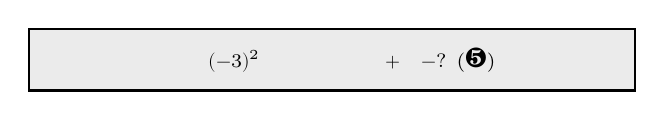
\begin{tikzpicture}[x=1cm, y=1cm, every node/.style={font=\scriptsize, text=black}]
    \draw[black, line width=0.9pt, fill=panelgray] (0,0) rectangle (7.7, 0.78);
    \node at (3.85, 0.39) {ផ្ទៀង៖ $(-3)^2$ មាននិទស្សន្តគូ តើចេញ $+$ ឬ $-$? (\cnum{5})};
  \end{tikzpicture}
  \end{center}
  \vspace{3pt}
  {\centering\fontsize{7.8pt}{10.5pt}\selectfont ហេតុផល / លេខ \cnum{1}--\cnum{5}៖ $\underline{\hspace{4.5cm}}$\par}
  \vfill
  \begin{tcolorbox}[enhanced, sharp corners, colback=panelgray, colframe=black, boxrule=0.8pt, boxsep=1pt, top=4pt, bottom=4pt, left=4pt, right=4pt]
    \centering\fontsize{8.5pt}{11.5pt}\selectfont
    \textbf{វិនិច្ឆ័យ៖} \quad \chkbox~ពិត (\ding{51}) \qquad \chkbox~ខុស (\ding{55})
  \end{tcolorbox}
\end{tcolorbox}

\vspace{7pt}

% --- ផ្នែកកាត់ទុកសម្រាប់គ្រូ (Teacher Remediation Key) & សំបុត្រចេញ ៣ សំណួរ ---
\noindent\scissors\ \dotfill\ \textbf{កាត់ទុកសម្រាប់គ្រូ (\en{Teacher Remediation Key}) \& សំបុត្រចេញ ៣ សំណួរ} \dotfill\ \scissors

\vspace{5pt}
\begin{tcolorbox}[
  enhanced, sharp corners, colback=panelgray, colframe=black,
  boxrule=0.95pt, boxsep=1pt, top=4pt, bottom=4pt, left=5pt, right=5pt
]
  \fontsize{7.55pt}{10.6pt}\selectfont
  \renewcommand{\arraystretch}{1.32}
  \begin{tabular}{|L{4.25cm}|L{4.25cm}|L{4.25cm}|L{4.25cm}|}
    \hline
    \cellcolor{headgray}\textbf{កាត \en{A} ៖ ខុស (\ding{55})} &
    \cellcolor{headgray}\textbf{កាត \en{B} ៖ ខុស (\ding{55})} &
    \cellcolor{headgray}\textbf{កាត \en{C} ៖ ត្រឹមត្រូវ (\ding{51})} &
    \cellcolor{headgray}\textbf{កាត \en{D} ៖ ខុស (\ding{55})} \\ \hline
    \textbf{ភ្លេចលើកភាគបែង (\cnum{1})!} \newline \textit{សួរភ្លាម៖} «$y^{-4}$ ស្ថិតក្នុងវង់ក្រចកដែរ — ត្រូវគណនា $(y^{-4})^2 = y^{-8}$!» &
    \textbf{បូកជំនួសគុណ (\cnum{3})!} \newline \textit{សួរភ្លាម៖} «$(y^{-4})^2$ ត្រូវគុណ $-4\times 2 = -8$ មិនមែន $-4+2$ ទេ!» &
    \textbf{ត្រឹមត្រូវ (\cnum{1}--\cnum{5})!} \newline $\dfrac{(-3)^2 (x^2)^2}{(y^{-4})^2} = \dfrac{9x^4}{y^{-8}} = 9x^4 y^8$ ($x,y\neq 0$)។ &
    \textbf{ខុសសញ្ញាគូ/សេស (\cnum{5})!} \newline \textit{សួរភ្លាម៖} «$-3$ នៅក្នុងវង់ក្រចកលើកស្វ័យគុណគូ $2$: $(-3)^2 = +9$!» \\ \hline
  \end{tabular}
\end{tcolorbox}

\vspace{5pt}
\begin{tcolorbox}[
  enhanced, sharp corners, colback=white, colframe=black,
  boxrule=0.95pt, boxsep=1pt, top=5pt, bottom=5pt, left=6pt, right=6pt
]
  \raggedright\fontsize{7.9pt}{11.6pt}\selectfont
  \textbf{សំបុត្រចេញ ៦០--៩០ វិនាទី (\en{Quick Exit Ticket} -- ៣ សំណួរ)៖}\quad ឈ្មោះ៖ $\underline{\hspace{3.6cm}}$ \quad ថ្នាក់៖ $\underline{\hspace{1.2cm}}$\\[4pt]
  \textbf{១) វង់ក្រចក \& សញ្ញា (\cnum{5})៖} គណនា $\left(\dfrac{-2a}{b^3}\right)^2 = \underline{\hspace{1.8cm}}$ \quad ធៀបនឹង \quad $-\left(\dfrac{2a}{b^3}\right)^2 = \underline{\hspace{1.8cm}}$ ($b\neq 0$)\\[4pt]
  \textbf{២) ផ្គុំបញ្ច្រាស (\cnum{1} ពីរទិស)៖} សរសេរជាស្វ័យគុណតែមួយ៖ $\dfrac{15^4}{3^4} = \left(\dfrac{\underline{\hspace{0.42cm}}}{\underline{\hspace{0.42cm}}}\right)^{\!\raisebox{-1.5pt}{\expbox}} = \underline{\hspace{0.9cm}}$\\[4pt]
  \textbf{៣) អន្ទាក់ \& ហេតុផល (\cnum{1}--\cnum{5})៖} តើ $\left(\dfrac{4+2}{2}\right)^2 = \dfrac{4^2+2^2}{2^2}$ ពិតឬទេ? \chkbox~ពិត \chkbox~ទេ \quad ព្រោះ៖ $\underline{\hspace{4.0cm}}$\\[3pt]
  \textit{\fontsize{7.3pt}{10.0pt}\selectfont (ចម្លើយគ្រូ៖ ១. $\frac{4a^2}{b^6}$ vs $-\frac{4a^2}{b^6}$; \quad ២. $(15/3)^4 = 5^4 = 625$; \quad ៣. ទេ — $3^2=9 \neq \frac{20}{4}=5$ ព្រោះស្វ័យគុណមិនចែកចាយលើ \en{+}!)}
\end{tcolorbox}

\clearpage

% ============================================================================
% ទំព័រទី ៦៖ ប័ណ្ណកិច្ចការផ្ទះ ជំហានទី ៥ — ២ ប័ណ្ណដូចគ្នាក្នុង ១ ទំព័រ A4 (ត្រូវគ្នា ១០០% នឹង LS_Plan_POWQ)
% ============================================================================
\pagebanner{សម្ភារៈទី ៦៖ ប័ណ្ណកិច្ចការផ្ទះ ជំហានទី ៥ \enbf{--} ២ ប័ណ្ណដូចគ្នាក្នុង ១ ទំព័រ \enbf{A4}}{ទំព័រ ៦/៦ \en{--} ជំហានទី ៥ (កាត់ ២ ប័ណ្ណ \scissors)}

\newcommand{\hwslipTwoPOWQ}[1]{%
\begin{tcolorbox}[
  enhanced, sharp corners, colback=white, colframe=white,
  borderline={1.0pt}{0pt}{black, dashed},
  boxsep=1pt, top=6pt, bottom=6pt, left=7pt, right=7pt
]
  \begin{tcolorbox}[
    enhanced, sharp corners, colback=headgray, colframe=black,
    boxrule=0.85pt, boxsep=1pt, top=3.5pt, bottom=3.5pt, left=6pt, right=6pt, after skip=6pt
  ]
    \fontsize{8.1pt}{11.2pt}\selectfont
    \textbf{\scissors\ កិច្ចការផ្ទះ (#1) \en{|} ២.៤.៣ ស្វ័យគុណនៃផលចែក \& លក្ខណៈទាំង ៣} \hfill \textbf{ចន្ទ ៧កើត កត្តិក ២៥៧០ \en{/} ១៦-១១-២០២៦}\\[2pt]
    ឈ្មោះសិស្ស៖ $\underline{\hspace{5.8cm}}$ \hspace{0.5cm} ថ្នាក់៖ $\underline{\hspace{1.8cm}}$ \hspace{0.5cm} លេខរៀង៖ $\underline{\hspace{1.4cm}}$
  \end{tcolorbox}

  \fontsize{8.3pt}{12.2pt}\selectfont
  \textbf{ផ្នែក ក (ទំ.១៨ \& ទំ.២៥ \en{\#6} គ) \en{--} ចុះលេខហេតុផល \cnum{1}--\cnum{5} ភ្ជាប់គ្រប់ជំហាន៖}\\[4pt]
  \hspace*{0.6em}\textbf{(១)} សម្រួល $\left(\dfrac{-3}{5}\right)^3 = \underline{\hspace{12.8cm}}$\\[5pt]
  \hspace*{0.6em}\textbf{(២)} សម្រួល $\left(\dfrac{2x^3 y^{-1}}{z^4}\right)^3 = \underline{\hspace{11.5cm}}$ ($y, z \neq 0$)\\[5pt]
  \hspace*{0.6em}\textbf{(៣)} គណនា $\left(\dfrac{4}{3}\right)^4\left(\dfrac{4}{3}\right)^{-6}\left(\dfrac{4}{3}\right)^3 = \underline{\hspace{11.2cm}}$

  \vspace{5pt}\hrule height 0.5pt\vspace{5pt}

  \fontsize{8.3pt}{12.2pt}\selectfont
  \textbf{ផ្នែក ខ (ទំ.២៥ \en{\#7} ង \& ទំ.២៦ \en{\#8} ក, គ)៖}\\[4pt]
  \hspace*{0.6em}\textbf{(១)} សម្រួល ($a,x \neq 0$)៖ $\dfrac{(32a^2x^8)^3}{(5ax)(-2a^2x^2)^2(-4a^3x)^3} = \underline{\hspace{10.1cm}}$\\[6pt]
  \hspace*{2.0em} $= \underline{\hspace{14.2cm}}$\\[5pt]
  \hspace*{0.6em}\textbf{(២)} សរសេរ $x^{12}$ ជាស្វ័យគុណនៃ $x^2$៖ $x^{12} = (\,x^2\,)^{\expbox[0.55cm]}$ \quad|\quad សរសេរ $2^{18}$ និង $(2^5)^6$ ជាស្វ័យគុណនៃ $8$៖\\[4pt]
  \hspace*{2.0em} $\bullet$ $2^{18} = (2^{\expbox})^{\expbox} = 8^{\expbox[0.50cm]}$ \hspace{1.4cm} $\bullet$ $(2^5)^6 = 2^{\expbox[0.50cm]} = (2^{\expbox})^{\expbox[0.50cm]} = 8^{\expbox[0.50cm]}$\\[5pt]
  \hspace*{0.6em}\chkbox\ \textbf{អានមុនមេរៀនបន្ទាប់៖} \textbf{៤.៤. ស្វ័យគុណនៃ \en{10}} (សៀវភៅគោល ទំ.១៩--២០) រួចសរសេរសំណួរ ១ ចំណុច។

  \vspace{5pt}
  \begin{tcolorbox}[
    enhanced, sharp corners, colback=panelgray, colframe=black,
    boxrule=0.75pt, boxsep=1pt, top=4pt, bottom=4pt, left=6pt, right=6pt
  ]
    \fontsize{7.7pt}{10.8pt}\selectfont
    \textbf{ផ្ទៀងខ្លួនឯង (\cnum{1}--\cnum{5})៖}
    \chkbox~ចុះលេខ \cnum{1}--\cnum{5} \en{|}
    \chkbox~សញ្ញាគូ/សេស $(-3)^3, (-2)^2, (-4)^3$ \en{|}
    \chkbox~ប្ដូរគោល $32=2^5,\; 8=2^3$! \hfill ហត្ថលេខា៖ $\underline{\hspace{2.1cm}}$
  \end{tcolorbox}
\end{tcolorbox}%
}

\vspace{3pt}
\hwslipTwoPOWQ{ប័ណ្ណទី ១}

\vspace{10pt}
\noindent\scissors\ \dotfill\ \textbf{កាត់តាមស្នាមចុចចែកជា ២ ប័ណ្ណ (\en{Cut Along Dashed Line})} \dotfill\ \scissors
\vspace{10pt}

\hwslipTwoPOWQ{ប័ណ្ណទី ២}

\end{document}
